\documentclass{article}
\usepackage{amsmath}
\usepackage{amssymb}
\usepackage[pdftex]{graphicx}
\usepackage[framed,numbered,autolinebreaks,useliterate]{mcode}
\lstset{breakatwhitespace=false}
\usepackage{pgfplots}

\pdfpagewidth 8.5in
\pdfpageheight 11in
\topmargin -1in
\headheight 0in
\headsep 0in
\textheight 8.5in
\textwidth 6.5in
\oddsidemargin 0in
\evensidemargin 0in 
\headheight 50pt
\headsep 0in
\footskip .75in

\title{STA 601 - Lab 5}
\author{Kedar Prabhudesai}
\date{October 3, 2013}

\begin{document}
\maketitle

{\Large\underline{\textbf{Multivariate Normal Density:}}}\\

Any p-Variate Normal Distribution can be expressed as follows:\\

$y \sim \mathcal{N}_p(\mu,\Sigma),$ $\mu = \left(\begin{matrix}\mu_1\\\mu_2\end{matrix}\right),$ $\Sigma = \left(\begin{matrix}\Sigma_{11}&\Sigma_{12}\\\Sigma_{21}&\Sigma_{22}\end{matrix}\right).$\\

The dimensions are given as follows:\\

$\mu_1 \rightarrow q \times 1$

$\mu_2 \rightarrow (p-q) \times 1$

$\Sigma_{11} \rightarrow q \times q$

$\Sigma_{12} \rightarrow q \times (p-q)$

$\Sigma_{21} \rightarrow (p-q) \times q$

$\Sigma_{22} \rightarrow (p-q) \times (p-q)$\\

The Conditional Distribution can be given as:\\

$(y_1 \mid y_2=a) \sim \mathcal{N}_q\left(\mu_1+\Sigma_{12}\Sigma_{22}^{-1}(a-\mu_2),\Sigma_{11}-\Sigma_{12}\Sigma_{22}^{-1}\Sigma_{21}\right)$\\

{\Large\underline{\textbf{Given Posterior:}}}\\

$\left(\begin{matrix}X\\Y\\Z\end{matrix}\right) \sim \mathcal{N}_3\left[\left(\begin{matrix}0\\0\\0\end{matrix}\right),\left(\begin{matrix}1&0.9&0.1\\0.9&1&0.1\\0.1&0.1&1\end{matrix}\right)\right]$\\

\pagebreak

\begin{enumerate}
\item {\underline{\textbf{Complete Conditionals:}}} Using the above equations we get the following parameters for the full conditionals:\\
$\mu_1 = 0,$
$\mu_2 = \left(\begin{matrix}0\\0\end{matrix}\right),$
$\Sigma_{11} = 1.$\\
\begin{itemize}
\item $X \mid Y,Z$\\
$\Sigma_{12} = \left(\begin{matrix}0.9&0.1\end{matrix}\right),$
$\Sigma_{21} = \left(\begin{matrix}0.9\\0.1\end{matrix}\right),$
$\Sigma_{22} = \left(\begin{matrix}1&0.1\\0.1&1\end{matrix}\right).$\\
\item $Y \mid X,Z$\\
$\Sigma_{12} = \left(\begin{matrix}0.9&0.1\end{matrix}\right),$
$\Sigma_{21} = \left(\begin{matrix}0.9\\0.1\end{matrix}\right),$
$\Sigma_{22} = \left(\begin{matrix}1&0.1\\0.1&1\end{matrix}\right).$\\
\item $Z \mid X,Y$\\
$\Sigma_{12} = \left(\begin{matrix}0.1&0.1\end{matrix}\right),$
$\Sigma_{21} = \left(\begin{matrix}0.1\\0.1\end{matrix}\right),$
$\Sigma_{22} = \left(\begin{matrix}1&0.9\\0.9&1\end{matrix}\right).$\\
\end{itemize}

\item {\underline{\textbf{Gibbs Sampler:}}} Algorithm:\\

Start with $\{Y^{(0)},Z^{(0)}\},$ 
\begin{itemize}
\item Draw $X^{(s+1)} \mid Y^{(s)},Z^{(s)},$\\
\item Draw $Y^{(s+1)} \mid X^{(s+1)},Z^{(s)},$\\
\item Draw $Z^{(s+1)} \mid X^{(s+1)},Y^{(s+1)}.$
\end{itemize}

\begin{center}
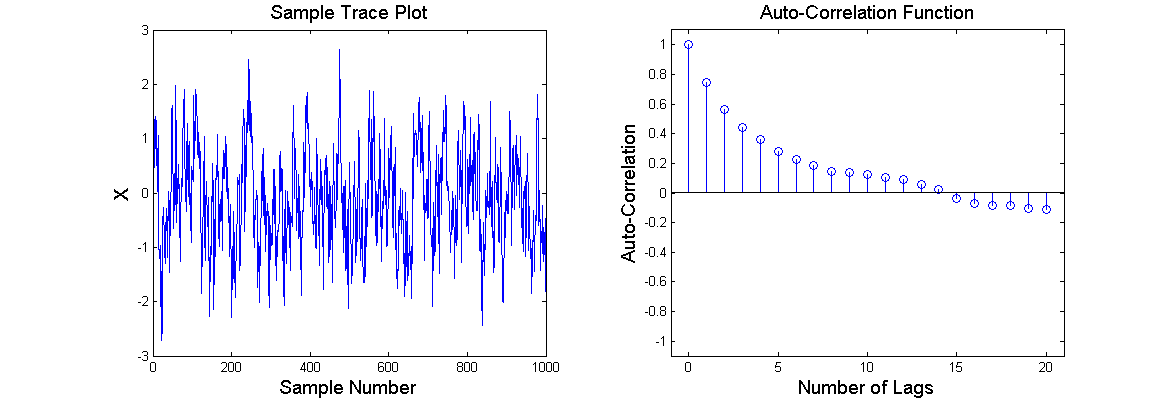
\includegraphics[scale=0.5]{FirstGibbsSampler.png}
\end{center}

\pagebreak

\item {\underline{\textbf{Gibbs Sampler with Block Updates:}}} The following are the parameters for conditional distributions:\\
\begin{itemize}
\item $X,Y \mid Z$\\
$\mu_1 = \left(\begin{matrix}0\\0\end{matrix}\right),$
$\mu_2 = 0.$\\
$\Sigma_{11} = \left(\begin{matrix}1&0.9\\0.9&1\end{matrix}\right),$
$\Sigma_{12} = \left(\begin{matrix}0.1\\0.1\end{matrix}\right),$
$\Sigma_{21} = \left(\begin{matrix}0.1&0.1\end{matrix}\right),$
$\Sigma_{22} = 1.$\\
\item $Z \mid X,Y$\\
$\mu_1 = 0$
$\mu_2 = \left(\begin{matrix}0\\0\end{matrix}\right),$\\
$\Sigma_{11} = 1,$
$\Sigma_{12} = \left(\begin{matrix}0.1&0.1\end{matrix}\right),$
$\Sigma_{21} = \left(\begin{matrix}0.1\\0.1\end{matrix}\right),$
$\Sigma_{22} = \left(\begin{matrix}1&0.9\\0.9&1\end{matrix}\right).$\\
\end{itemize}

Gibbs Sampling Algorithm:\\

Start with $\{Z^{(0)}\},$ 
\begin{itemize}
\item Draw $\{X^{(s+1)},Y^{(s+1)}\} \mid Z^{(s)},$\\
\item Draw $Z^{(s+1)} \mid \{X^{(s+1)},Y^{(s+1)}\}.$
\end{itemize}

\begin{center}
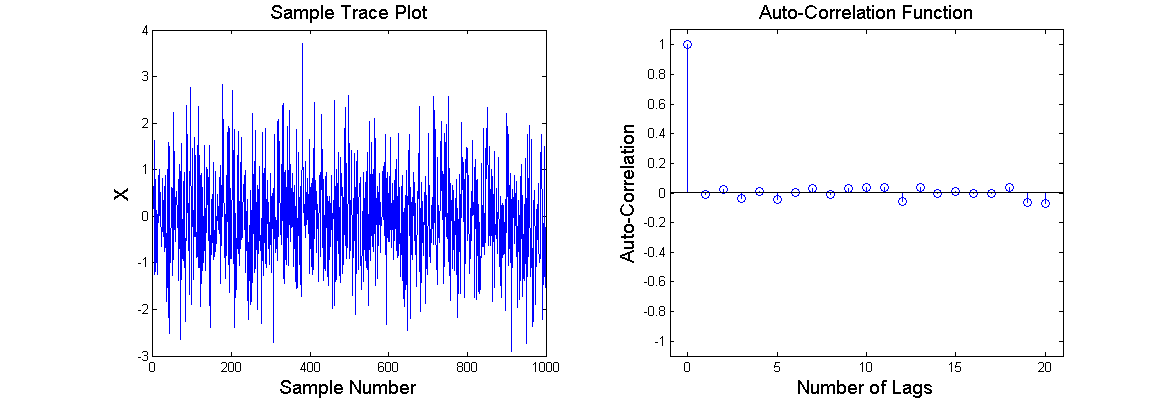
\includegraphics[scale=0.5]{SecondGibbsSampler.png}
\end{center}

\pagebreak

\item {\underline{\textbf{Comparison between the two Samplers:}}} From the autocorrelation plots, we can see that the second chain clearly mixes better than the first one. From the covariance matrix we see that $X,Y$ and very highly correlated ($\rho=0.9$) which are both poorly correlated with $Z$ ($\rho=0.1$). We know that consecutive samples from Gibbs Sampler are highly correlated.\\

In the first sampler we draw $X$ and $Y$ from their conditional distributions. Since, they are highly correlated, each $X$ sample is now not only correlated with its previous sample but also with its $Y$ sample. This is why it takes time for the first chain to converge.\\

In the second chain, we draw samples from the $X,Y$ joint distribution, we avoid the inter variable correlation. Also since $Z$ is poorly correlated with $X$ and $Y$, we get good mixing.\\

This can be further explained using the following figures. Here I dropped the correlation between $X$ and $Y$ to $\rho=0.15.$ In this case both samplers show good mixing.\\
\end{enumerate}

\begin{center}
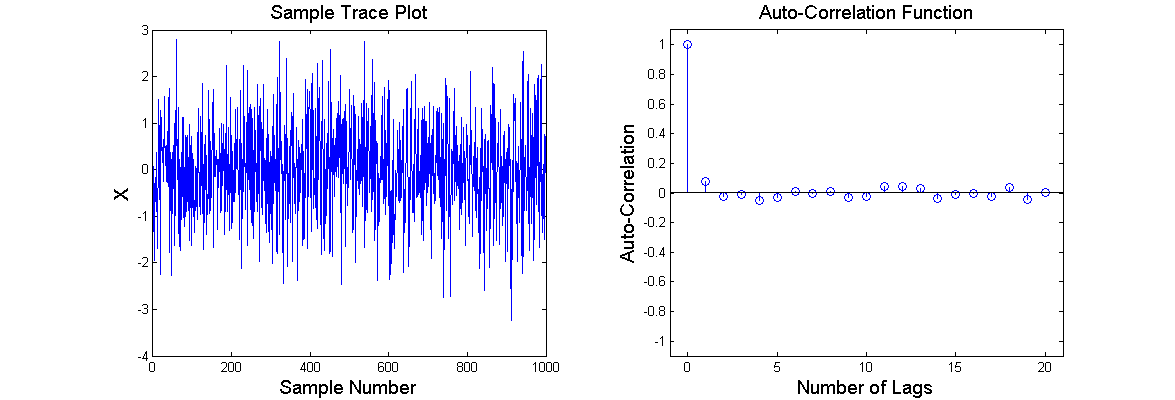
\includegraphics[scale=0.5]{FirstGibbsSamplerLessCorr.png}
\end{center}
\begin{center}
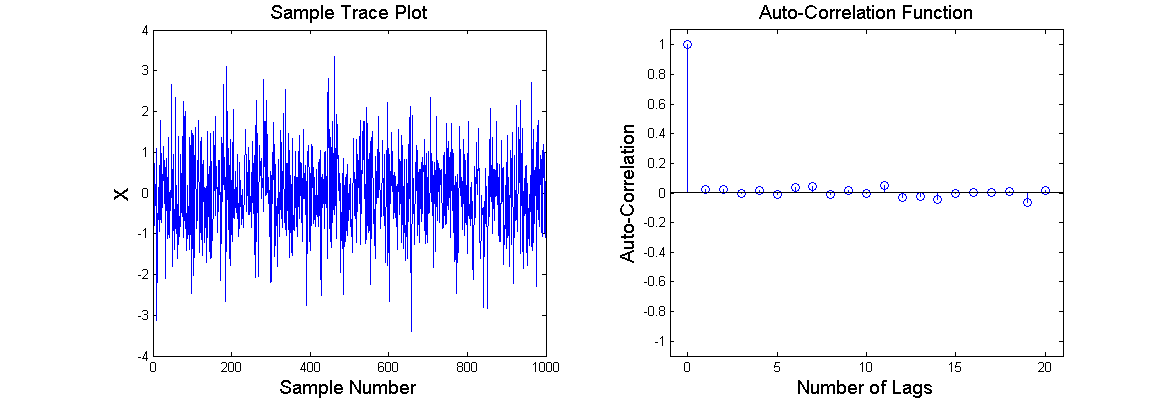
\includegraphics[scale=0.5]{SecondGibbsSamplerLessCorr.png}
\end{center}

\pagebreak
\noindent {\Large\underline{\textbf{Appendix:}}}\\
\lstinputlisting{C:/Users/ksp6/Documents/Classes/2013-Fall/STA601-BayesAndModStats/labs/lab5/sta601_ksp6_Lab5.m}

\end{document}